\part*{Appendix}


\subsection*{Simulated Experiments}


\begin{wrapfigure}{r}{.34\columnwidth}
	\centering
	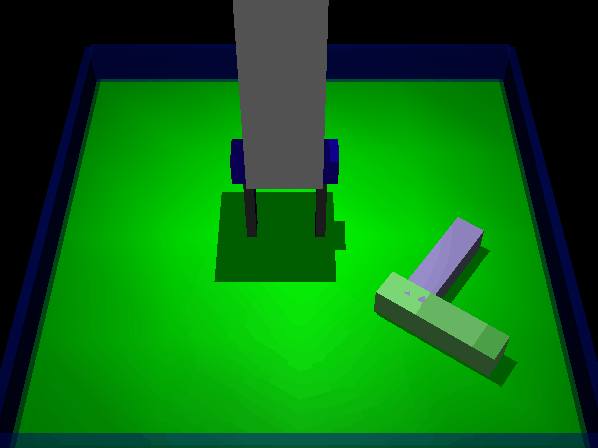
\includegraphics[width=0.3\columnwidth]{images/simulator.png}
	\caption{\small{Block pushing simulator}}
	\label{fig:sim}
\end{wrapfigure}

In order to provide a more controlled comparison, we also set up a realistic simulation environment using MuJoCo \cite{todorov2012mujoco}, which includes a robotic manipulator controlled via Cartesian position control, similar to our real world setup, pushing randomly-generated L-shaped objects with random colors (see details in supplementary materials). 
We trained the same video prediction model in this environment, and set up 50 evaluation tasks where blocks must be pushed to target locations with maximum episode lengths of 120 steps. 
\begin{wrapfigure}{r}{.4\columnwidth}
	\centering
	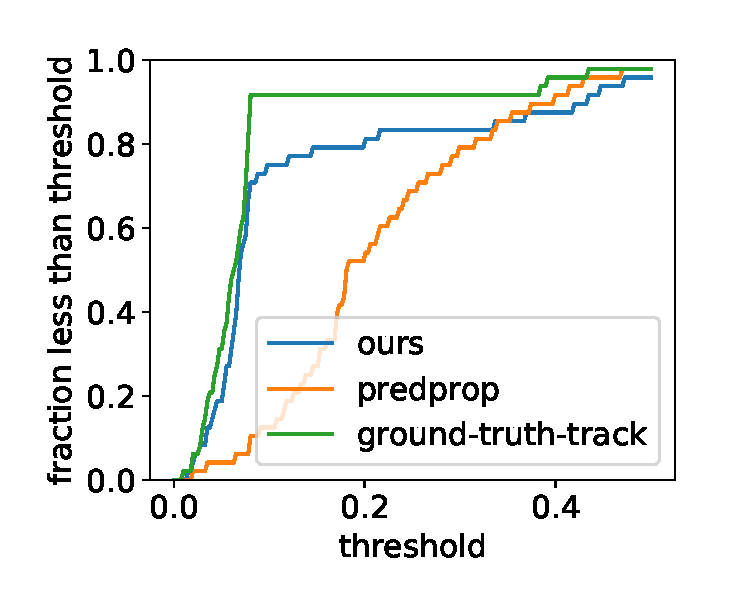
\includegraphics[width=0.4\columnwidth]{images/2obj_scores_ours-predprop-ground-truth-track.pdf}
	\caption{\small{Simulated evaluation. Fraction of trajectories with final object distance lower than threshold (higher is better).}}
	\label{fig:sim_bench}
\end{wrapfigure} 


We  compare our proposed registration-based method, ``predictor propagation,'' and ground-truth registration obtained from the simulator, which provides an oracle upper bound on registration performance. \autoref{fig:sim_bench} shows the results of this simulated evaluation, where the x-axis shows different distance thresholds, and the y-axis shows the fraction of evaluation scenarios where each method pushed the object within that threshold. We can see that, for thresholds around 0.1, our method drastically outperforms predictor propagation (i.e., prior work~\cite{sna}), and has a relatively modest gap in performance against ground-truth tracking. This indicates that our registration method is highly effective in guiding visual MPC, despite being entirely self-supervised.

In our simulated experiments, we use end-effector position control with the arm illustrated in Figure~\ref{fig:sim}. In this environment, the video prediction model was trained with using 60,000 training trajectories.

\section*{Planner Implementation Details}

We use the cross-entropy method \cite{cem-rk-13} to optimize the action sequence with respect to the cost function. At the first iteration 400 samples and at later iterations 200 samples are taken and  a Gaussian is fitted to the best $5\%$ of the samples. We use 3 CEM iterations. The length of the prediction horizon is 15, to reduce the search space we use an action repeat of 3, so that only a sequence of 5 independent actions needs to be optimized. Since the action space is 4 (x,y,z,rotation) a total of 20 variables are optimized.

\section*{Improvements to online optimization procedure}
In the visual MPC setting the action sequences found by the optimizer can be very different between execution times steps (not to be confused with prediction time steps). For example at one time step the optimizer might find a pushing action leading towards the goal and in the next time step it determines a grasping action to the optimal to reach the goal. Naive replanning at every time step can result in alternating between a pushing attempt and a grasping attempt indefinitely causing the agent to get stuck and not making any progress towards to goal. 

We show that we can resolve this problem by modifying the sampling distribution of the first iteration of CEM so that the optimizer commits to the plan found in the previous time step. In prior work \cite{sna} the sampling distribution at first iteration of CEM is chosen to be a Gaussian with diagonal covariance matrix and zero mean. We instead use the best action sequence found in the optimization of the previous time step as the mean. Since this action sequence is optimized for the previous time step we only use the values $a_{1:T}$ and omit the first action, where $T$ is the prediction horizon. To sample actions close to the action sequence from the previous time step we reduce the entries of the diagonal covariance matrix for the first $T-1$ time steps. It is crucial that the last entry of the covariance matrix at the end of the horizon is not reduced otherwise no exploration could happen for the last time step causing poor performance at later time steps.